\documentclass[11pt]{article}
% =====================================================================
%  preamble.tex  --  SHARED PREAMBLE FOR CS-4031 COMPILER CONSTRUCTION
%  Fall 2026, FAST-NU Lahore
% =====================================================================

% ---------- Page geometry ----------
\usepackage[a4paper, margin=2.2cm, headsep=14pt, footskip=28pt]{geometry}

% ---------- Fonts / encoding ----------
\usepackage[utf8]{inputenc}
\usepackage[T1]{fontenc}

% ---------- Math ----------
\usepackage{amsmath, amssymb, amsthm}

% ---------- Colors ----------
\usepackage[table]{xcolor}
\definecolor{nuNavy}{HTML}{102A43}      % primary heading color
\definecolor{nuBlue}{HTML}{1B5FA8}      % accent / links
\definecolor{nuLight}{HTML}{EAF2FB}     % light panel background
\definecolor{dbGreen}{HTML}{1F7A4D}     % "Dragon Book / examinable" boxes
\definecolor{dbGreenBg}{HTML}{EAF7EF}
\definecolor{enrichGold}{HTML}{9A6A00}  % "enrichment / beyond DB" boxes
\definecolor{enrichGoldBg}{HTML}{FFF6E0}
\definecolor{examRed}{HTML}{B3261E}     % "exam focus" boxes
\definecolor{examRedBg}{HTML}{FCEBEA}
\definecolor{histPurple}{HTML}{5B3A8E}
\definecolor{histPurpleBg}{HTML}{F2EBFB}
\definecolor{takeawayTeal}{HTML}{0F6F6A}
\definecolor{takeawayTealBg}{HTML}{E7F6F5}
\definecolor{lightgray}{HTML}{F5F5F5}

% ---------- Headers / footers ----------
\usepackage{fancyhdr}
\pagestyle{fancy}
\fancyhf{}
\renewcommand{\headrulewidth}{0.6pt}
\renewcommand{\footrulewidth}{0.3pt}
\fancyhead[L]{\small\sffamily\color{nuNavy} CS-4031 Compiler Construction}
\fancyhead[R]{\small\sffamily\color{nuNavy} \rightmark}
\fancyfoot[L]{\small\sffamily\color{gray} FAST-NU Lahore, Fall 2026}
\fancyfoot[C]{\small\sffamily\color{gray} \thepage}
\fancyfoot[R]{\small\sffamily\color{gray} Notes by course staff}

% ---------- Section styling ----------
\usepackage{titlesec}
\titleformat{\section}
  {\normalfont\Large\bfseries\color{nuNavy}}
  {\thesection}{0.6em}{}
\titleformat{\subsection}
  {\normalfont\large\bfseries\color{nuBlue}}
  {\thesubsection}{0.6em}{}
\titlespacing*{\section}{0pt}{1.4em}{0.8em}
\titlespacing*{\subsection}{0pt}{1.1em}{0.5em}

% ---------- Lists, tables, misc ----------
\usepackage{enumitem}
\setlist{topsep=4pt, itemsep=2pt, parsep=0pt}
\usepackage{array, booktabs, tabularx, longtable, multirow}
\usepackage{graphicx}
\usepackage{tikz}
\usetikzlibrary{arrows.meta, positioning, shapes.geometric, fit, backgrounds, calc}
\usepackage{float}
\usepackage[colorlinks=true, linkcolor=nuBlue, citecolor=nuBlue, urlcolor=nuBlue]{hyperref}

% ---------- Table-of-contents number width ----------
% Default article.cls reserves just enough horizontal space in the TOC for a
% single-digit section number. Once any lecture grows past 9 top-level
% sections (as a merged/longer lecture can), two-digit numbers like "3.10"
% collide visually with the title text right after them ("3.10Extensions").
% tocloft lets us widen that reserved space once, here, so every lecture
% is protected regardless of how many sections it ends up with.
\usepackage{tocloft}
\setlength{\cftsecnumwidth}{2.8em}
\setlength{\cftsubsecnumwidth}{3.4em}
\renewcommand{\theHsection}{L\thelecnum.\arabic{section}}
\renewcommand{\theHsubsection}{L\thelecnum.\arabic{section}.\arabic{subsection}}
\renewcommand{\theHsubsubsection}{L\thelecnum.\arabic{section}.\arabic{subsection}.\arabic{subsubsection}}

% ---------- Cross-reference machinery (no hard-coded section/lecture numbers) ----------
% Every lecture resets \setcounter{section}{0} at its own top (see \lecturemeta / the
% \setcounter{section}{0} call in each lecture file), so within a single lecture, sections
% would normally print as a bare "1", "2", "3", ... -- indistinguishable at a glance from the
% *next* lecture's own "1", "2", "3", ... once everything is stitched into one combined PDF.
% Prefixing the *displayed* section number with the lecture number fixes this without touching
% any individual lecture file: "3.2" unambiguously means "Lecture 3, Section 2" everywhere,
% including in the combined table of contents.
\renewcommand{\thesection}{\thelecnum.\arabic{section}}

% \Sref{<label>} is the standard way to refer to a section from prose, in place of typing a
% literal number. Pair every \section/\subsection that is ever referred to elsewhere with a
% \label{sec:...} right after it, then write \Sref{sec:...} wherever the old text would have
% hard-coded "\S2.4" or similar. If the numbering ever shifts (a new section inserted, content
% reordered), every \Sref pointing at that label updates automatically on the next compile.
\newcommand{\Sref}[1]{\S\ref{#1}}


% ---------- Box framework (tcolorbox) ----------
\usepackage[most]{tcolorbox}
\tcbuselibrary{skins, breakable}

\newtcolorbox{lecbox}[3]{
  breakable, enhanced, sharp corners=downhill,
  colback=#2, colframe=#1,
  boxrule=0.6pt, left=6pt, right=6pt, top=4pt, bottom=4pt,
  fonttitle=\bfseries\sffamily, coltitle=white,
  colbacktitle=#1,
  title={#3},
  attach boxed title to top left={yshift=-0.3mm, xshift=2mm},
  boxed title style={sharp corners, colframe=#1, boxrule=0pt},
  top=8mm
}

\newenvironment{coreidea}[1][Core Idea (Dragon Book)]
  {\begin{lecbox}{dbGreen}{dbGreenBg}{#1}}
  {\end{lecbox}}

\newenvironment{examfocus}[1][Exam Focus]
  {\begin{lecbox}{examRed}{examRedBg}{#1}}
  {\end{lecbox}}

\newenvironment{enrichment}[1][Beyond the Dragon Book -- Enrichment]
  {\begin{lecbox}{enrichGold}{enrichGoldBg}{#1}}
  {\end{lecbox}}

\newenvironment{historynote}[1][A Bit of History]
  {\begin{lecbox}{histPurple}{histPurpleBg}{#1}}
  {\end{lecbox}}

\newenvironment{takeaways}[1][Key Takeaways]
  {\begin{lecbox}{takeawayTeal}{takeawayTealBg}{#1}}
  {\end{lecbox}}

\newtcolorbox{defbox}[1]{
  breakable, enhanced, colback=nuLight, colframe=nuBlue,
  boxrule=0.5pt, left=6pt, right=6pt, top=3pt, bottom=3pt,
  fonttitle=\bfseries, coltitle=nuNavy,
  title={Definition: #1}
}
\newtcolorbox{examplebox}[1]{
  breakable, enhanced, colback=white, colframe=gray!60,
  boxrule=0.5pt, left=6pt, right=6pt, top=3pt, bottom=3pt,
  fonttitle=\bfseries, coltitle=black,
  title={Example: #1}
}

% ---------- Lecture metadata machinery ----------
\newcommand{\thelecnum}{}
\newcommand{\lecshorttitle}{}
\newcommand{\lecclo}{}
\newcommand{\lecdbrefs}{}
\newcommand{\lecotherrefs}{}
\newcommand{\lecfulltitle}{}

\newcommand{\lecturemeta}[5]{%
  \global\renewcommand{\thelecnum}{#1}%
  \global\renewcommand{\lecfulltitle}{#2}%
  \global\renewcommand{\lecclo}{#3}%
  \global\renewcommand{\lecdbrefs}{#4}%
  \global\renewcommand{\lecotherrefs}{#5}%
}
\newcommand{\lecshort}[1]{%
  \global\renewcommand{\lecshorttitle}{#1}%
  \markright{Lecture \thelecnum\ --- #1}%
}

% ---------- Per-lecture \label and table-of-contents entry ----------
% \lecturelabel defines \label{lec:<N>} so other lectures can write "Lecture~\ref{lec:5}"
% instead of a hard-coded "Lecture 5" that silently goes stale if lectures are ever
% renumbered or reordered. \label normally captures whatever \thesection/\thechapter/etc.
% last set as \@currentlabel; since a bare lecture title isn't a sectioning command, we set
% \@currentlabel to \thelecnum ourselves first, so \ref{lec:<N>} prints just the number.
% \makeatletter/\makeatother are required here: \@currentlabel contains "@", which is not a
% letter by default in a plain \input file like this one (only inside .cls/.sty loading does
% LaTeX make that automatic) -- without this, "\@currentlabel" tokenizes as the unrelated
% control-symbol "\@" followed by the literal word "currentlabel", silently missing the
% kernel's real \@currentlabel entirely and leaving every \ref{lec:...} blank.
\makeatletter
\newcommand{\lecturelabel}{%
  \global\edef\@currentlabel{\thelecnum}%
  \label{lec:\thelecnum}%
}
\makeatother

% \lecturetocentry inserts one bold, page-level line into the *combined* table of contents
% for this lecture, at the same outline depth LaTeX normally reserves for \part -- one level
% above \section. This is what turns the combined TOC from a flat, ambiguous run of
% "1, 2, 3, 1, 2, 3, 4, ..." into a clearly hierarchical "Lecture 1: <title> / 1.1 ... / 1.2
% ... // Lecture 2: <title> / 2.1 ... / ...". It only affects the TOC listing -- it does not
% print a page break or heading in the body, since \makelecturetitle already provides that.
\newcommand{\lecturetocentry}{%
  \phantomsection
  \addcontentsline{toc}{part}{Lecture \thelecnum: \lecshorttitle}%
}

\newcommand{\makelecturetitle}{%
  \lecturelabel
  \lecturetocentry
  \begin{center}
    {\small\sffamily\color{gray} THE NATIONAL UNIVERSITY OF COMPUTER AND EMERGING SCIENCES, LAHORE}\\[2pt]
    {\small\sffamily\color{gray} CS-4031 Compiler Construction --- Fall 2026}\\[10pt]
    {\Huge\bfseries\color{nuNavy} Lecture \thelecnum}\\[4pt]
    {\LARGE\bfseries\color{nuBlue} \lecfulltitle}
  \end{center}
  \vspace{6pt}
  \noindent
  \begin{tcolorbox}[breakable, enhanced, colback=nuLight, colframe=nuNavy,
      boxrule=0.6pt, left=8pt, right=8pt, top=4pt, bottom=4pt]
    \small
    \begin{tabularx}{\textwidth}{@{}l X@{}}
      \textbf{CLO(s) covered:} & \lecclo \\
      \textbf{Dragon Book [DB]:} & \lecdbrefs \\
      \textbf{Other references:} & \lecotherrefs \\
    \end{tabularx}
  \end{tcolorbox}
  \vspace{4pt}
}

\newcommand{\beyonddb}{\textcolor{enrichGold}{\small\textbf{[beyond DB]}}\ }
\newcommand{\dbtag}{\textcolor{dbGreen}{\small\textbf{[DB]}}\ }

% ---------- Bibliography convention ----------
% Each lecture file ends its own "References for This Lecture" section with a
% \begin{thebibliography}{99} ... \end{thebibliography} block (no external .bib file or
% bibtex pass needed -- \cite{} resolves against \bibitem entries in the same document via
% the normal two-pass pdflatex + .aux mechanism already used for every other cross-reference
% here). A lecture only lists the \bibitem entries it actually \cite{}s.
%
% To keep citation keys consistent as more lectures are added, reuse these canonical keys
% (and the same canonical \bibitem text) rather than inventing new ones for the same source:
%   db        Aho, Lam, Sethi, Ullman -- Compilers: Principles, Techniques, and Tools (2nd ed.)
%   et        Cooper & Torczon -- Engineering a Compiler (2nd ed.)
%   ap        Appel -- Modern Compiler Implementation in C/Java/ML
%   pp        Scott -- Programming Language Pragmatics
%   mu        Muchnick -- Advanced Compiler Design and Implementation
%   an        Parr -- The Definitive ANTLR 4 Reference
%   gr        Gries -- Compilers: A Survey
%   llvmlangref   LLVM Language Reference Manual
%   llvmka        "My First Language Frontend with LLVM" (Kaleidoscope Tutorial)
%   antlrsite     ANTLR4 project site
%   tssite        Tree-sitter site
%   mlir          Lattner et al., "MLIR: A Compiler Infrastructure for the End of Moore's Law"
%   mlirdocs      The MLIR Project, official documentation
% A "Citation ... multiply defined" warning in the combined full-course-notes.pdf build (when
% two lectures both cite, say, \bibitem[DB]{db}) is expected and harmless: each lecture's own
% thebibliography block is independent, the canonical text is identical everywhere it is
% reused, and the explicit [DB]-style label (not an auto-generated number) is what actually
% gets printed, so it renders identically regardless of which instance "wins" in the aux file.


\lecturemeta{1}
  {Compilers vs.\ Interpreters vs.\ JIT; Why Study Compilers; Applications of Compiler Technology}
  {CLO 1}
  {\S1.1 (Language Processors), \S1.4 (Language-Processing Systems: compiler/interpreter distinction), \S1.5 (Applications of Compiler Technology)}
  {[ET] Engineering a Compiler \S1.1; [AP] Modern Compiler Implementation, Ch.\,1}
\lecshort{Compilers, Interpreters \& JIT}

\begin{document}
\makelecturetitle

\begin{coreidea}[Lecture Roadmap]
\begin{enumerate}
  \item What is a language processor, and what exactly is a \emph{compiler}?
  \item Compilers vs.\ interpreters vs.\ just-in-time (JIT) compilation --- three ways to run a program.
  \item Why study compilers at all, even if you never write one professionally?
  \item Applications of compiler technology far beyond ``turning C into an executable.''
\end{enumerate}
This lecture is entirely conceptual --- no algorithms yet. Lecture 2 covers the internal
\emph{structure} (phases) of a compiler in detail.
\end{coreidea}

\section{What Is a Language Processor?}

\dbtag A \textbf{language processor} is any program that takes another program written in
some source notation and does something useful with it --- runs it, translates it, checks it,
or transforms it. Compilers are the most famous member of this family, but not the only one.

\begin{defbox}{Compiler}
A \textbf{compiler} is a program that reads a program written in one language --- the
\emph{source language} --- and translates it into an equivalent program in another language ---
the \emph{target language}. Along the way, if the source program has errors, the compiler
should report them to the user in a useful way.
\end{defbox}

Two things are packed into that definition and worth pulling apart, because exam questions love
to test exactly this distinction:

\begin{itemize}
  \item \textbf{Translation, not execution.} A compiler's job is to \emph{produce} a target
  program. It does not itself run your code. If you compile \texttt{main.c} with GCC, GCC's job
  ends when it hands you \texttt{a.out}; a completely different program (the operating system's
  loader, then the CPU) is what actually executes it.
  \item \textbf{Equivalence.} The target program must have the same meaning as the source
  program. This is the single hardest engineering promise a compiler makes, and essentially the
  entire field of compiler optimization exists to preserve this promise while still making the
  target program faster.
\end{itemize}

\begin{center}
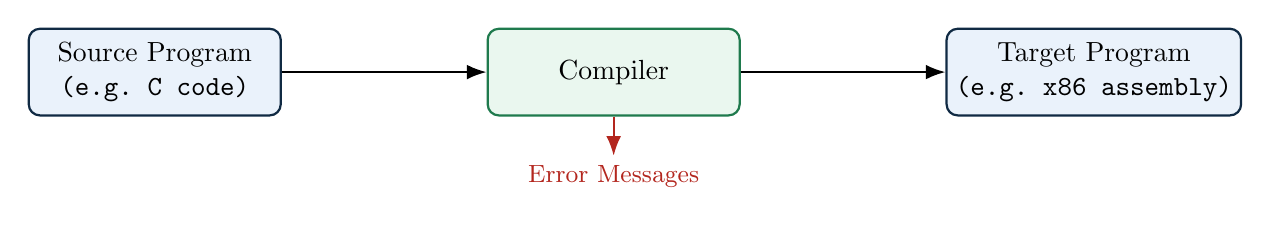
\begin{tikzpicture}[
  box/.style={draw, thick, rounded corners, minimum height=1.1cm, minimum width=3.2cm, align=center, fill=nuLight, draw=nuNavy},
  lbl/.style={font=\small\itshape}
]
  \node[box] (src) {Source Program\\\texttt{(e.g.\ C code)}};
  \node[box, fill=dbGreenBg, draw=dbGreen, right=2.6cm of src] (comp) {Compiler};
  \node[box, right=2.6cm of comp] (tgt) {Target Program\\\texttt{(e.g.\ x86 assembly)}};
  \node[below=0.5cm of comp, font=\small, text=examRed] (err) {Error Messages};

  \draw[-{Latex[length=2.5mm]}, thick] (src) -- (comp);
  \draw[-{Latex[length=2.5mm]}, thick] (comp) -- (tgt);
  \draw[-{Latex[length=2.5mm]}, thick, examRed] (comp) -- (err);
\end{tikzpicture}
\end{center}

\begin{examfocus}
Be able to state, in one sentence, that a compiler \emph{translates}; it does not
\emph{execute}. A one-line definition question like ``define a compiler'' is a classic
first-quiz question and students routinely lose marks by describing what an interpreter does
instead.
\end{examfocus}

\section{Compilers vs.\ Interpreters vs.\ JIT Compilation}

This is the heart of today's lecture (DB \S1.4). There are three broad strategies for getting
from source code to a running program, and almost every real language-processing system you use
day to day is one of these three, or (very commonly) a hybrid.

\subsection{Pure Compilation (Ahead-of-Time)}

\dbtag The compiler translates the entire source program into target-machine code \emph{before}
execution begins. The target program can then be run any number of times, independently of the
compiler. C, C++, Rust, and (classic) Fortran compilers work this way.

\begin{center}
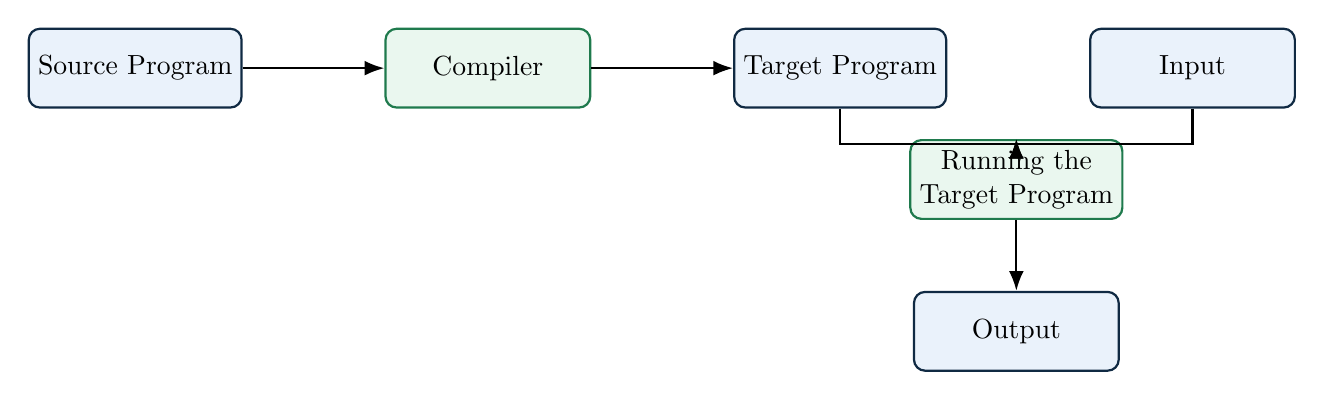
\begin{tikzpicture}[
  box/.style={draw, thick, rounded corners, minimum height=1cm, minimum width=2.6cm, align=center},
  phase/.style={box, fill=dbGreenBg, draw=dbGreen},
]
  \node[box, fill=nuLight, draw=nuNavy] (src) {Source Program};
  \node[phase, right=1.8cm of src] (comp) {Compiler};
  \node[box, fill=nuLight, draw=nuNavy, right=1.8cm of comp] (tgt) {Target Program};
  \node[box, fill=nuLight, draw=nuNavy, right=1.8cm of tgt] (input) {Input};
  \node[box, fill=dbGreenBg, draw=dbGreen, below=0.9cm of $(tgt)!0.5!(input)$] (run) {Running the\\Target Program};
  \node[box, fill=nuLight, draw=nuNavy, below=0.9cm of run] (out) {Output};

  \draw[-{Latex[length=2.5mm]}, thick] (src) -- (comp);
  \draw[-{Latex[length=2.5mm]}, thick] (comp) -- (tgt);
  \draw[-{Latex[length=2.5mm]}, thick] (tgt.south) -- ++(0,-0.45) -| (run.north);
  \draw[-{Latex[length=2.5mm]}, thick] (input.south) -- ++(0,-0.45) -| (run.north);
  \draw[-{Latex[length=2.5mm]}, thick] (run) -- (out);
\end{tikzpicture}
\end{center}

\textbf{Trade-off:} compilation itself can be slow and happens ``offline,'' but every run of the
target program afterward is fast, because all the translation work has already been paid for.

\subsection{Pure Interpretation}

\dbtag An \textbf{interpreter} does not produce a separate target program at all. Instead, it
directly executes the operations specified in the source program, using the source program (or a
close representation of it) as input on every single run.

\begin{defbox}{Interpreter}
An interpreter is a language processor that reads a source program and, using the input
supplied by the user, \emph{directly} produces the output of that program --- with no separate
translation phase that produces standalone target code the user can run independently.
\end{defbox}

\begin{center}
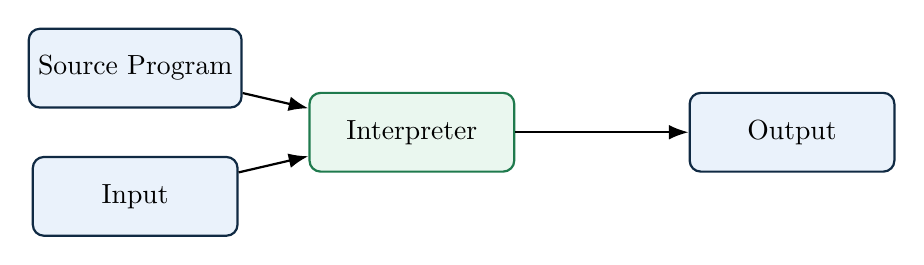
\begin{tikzpicture}[
  box/.style={draw, thick, rounded corners, minimum height=1cm, minimum width=2.6cm, align=center, fill=nuLight, draw=nuNavy},
  phase/.style={box, fill=dbGreenBg, draw=dbGreen},
]
  \node[box] (src) {Source Program};
  \node[box, below=0.6cm of src] (input) {Input};
  \node[phase, right=2.2cm of $(src)!0.5!(input)$] (interp) {Interpreter};
  \node[box, right=2.2cm of interp] (out) {Output};

  \draw[-{Latex[length=2.5mm]}, thick] (src) -- (interp);
  \draw[-{Latex[length=2.5mm]}, thick] (input) -- (interp);
  \draw[-{Latex[length=2.5mm]}, thick] (interp) -- (out);
\end{tikzpicture}
\end{center}

Classic (older) Python, shell scripts, and simple Basic interpreters are close to this pure
model: the interpreter re-examines and re-dispatches on the source (or its parsed form) every
single time a statement executes, even inside a loop that runs a million times.

\textbf{Trade-off:} there is no separate compile step, so you can start running --- and get
feedback on --- code instantly, which is wonderful for interactive development and REPLs. The
cost is repeated re-interpretation overhead every time the same line of code runs, which DB
notes can make interpretation \textbf{10--100$\times$ slower} than running compiled code.

\begin{examfocus}
Know this speed trade-off in both directions: compilation trades slower ``build time'' for
faster ``run time''; interpretation trades away build time for slower, but more flexible and
immediate, run time. Also know that \emph{portability} is a classic interpreter advantage: the
same source runs unmodified on any machine that has the interpreter, with no separate compile
step per target machine.
\end{examfocus}

\subsection{The Hybrid Reality: Bytecode + JIT}

\beyonddb In practice, almost no serious modern language is \emph{purely} compiled or
\emph{purely} interpreted. DB \S1.4 briefly mentions Java's model as a hybrid; it is worth
understanding this hybrid model properly, because it is how the overwhelming majority of code
you run today --- Java, C\#, JavaScript, modern Python (via PyPy), and even Python's own CPython
--- actually executes.

\begin{enumerate}
  \item \textbf{Source $\to$ bytecode.} A ``front-end'' compiler translates source code into a
  compact, machine-independent intermediate form called \textbf{bytecode} (Java's \texttt{.class}
  files hold JVM bytecode; Python's \texttt{.pyc} files hold Python bytecode).
  \item \textbf{Bytecode $\to$ execution.} A \textbf{virtual machine (VM)} then runs this
  bytecode. It can do this two ways:
  \begin{itemize}
    \item \emph{Interpret} the bytecode directly, instruction by instruction (slow but starts
    instantly) -- this is what most bytecode VMs do at first.
    \item \emph{Just-in-time (JIT) compile} hot pieces of bytecode --- the loops and functions
    that run over and over --- into native machine code \emph{while the program is running}, and
    cache that native code for reuse.
  \end{itemize}
\end{enumerate}

\begin{defbox}{Just-In-Time (JIT) Compilation}
JIT compilation defers translation to native machine code until run time, and does so
selectively: only code that is actually hot (executed frequently) is compiled, while cold code
may remain interpreted. This lets a system get the fast startup of an interpreter and the fast
steady-state speed of a compiler.
\end{defbox}

\begin{examplebox}{Tiered execution in real systems}
\begin{itemize}
  \item \textbf{JVM (HotSpot):} interprets bytecode first; the C1 (``client'') JIT compiles warm
  methods quickly with light optimization; the C2 (``server'') JIT recompiles the hottest methods
  with heavy optimization once enough profiling data exists.
  \item \textbf{V8 (Chrome/Node.js JavaScript engine):} \texttt{Ignition} interprets bytecode;
  \texttt{Sparkplug} does a fast baseline JIT; \texttt{TurboFan} does an aggressive optimizing
  JIT for hot functions, and can \emph{deoptimize} back to the interpreter if an assumption used
  for optimization (e.g.\ ``this variable is always a number'') turns out to be wrong.
  \item \textbf{CPython (standard Python):} traditionally a pure bytecode interpreter with no
  JIT; \texttt{PyPy} is an alternative Python implementation that adds a JIT and is often
  5--10$\times$ faster on long-running code as a result.
\end{itemize}
\end{examplebox}

\begin{center}
\resizebox{\textwidth}{!}{%
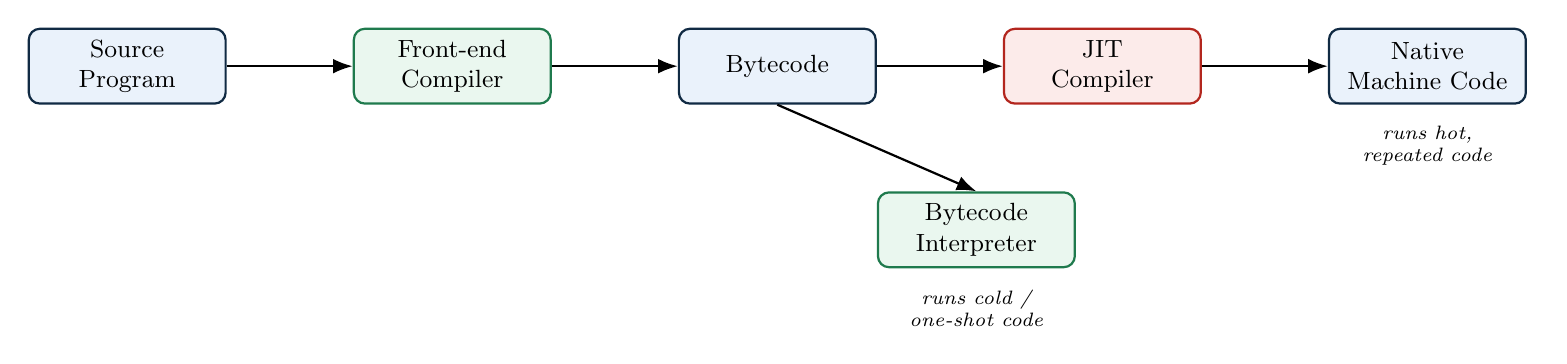
\begin{tikzpicture}[
  box/.style={draw, thick, rounded corners, minimum height=0.95cm, minimum width=2.5cm, align=center, fill=nuLight, draw=nuNavy, font=\small},
  phase/.style={box, fill=dbGreenBg, draw=dbGreen},
  hot/.style={box, fill=examRedBg, draw=examRed},
]
  \node[box] (src) {Source\\Program};
  \node[phase, right=1.6cm of src] (fe) {Front-end\\Compiler};
  \node[box, right=1.6cm of fe] (bc) {Bytecode};
  \node[phase, below right=1.1cm and 0.0cm of bc] (vm) {Bytecode\\Interpreter};
  \node[hot, right=1.6cm of bc] (jit) {JIT\\Compiler};
  \node[box, right=1.6cm of jit] (native) {Native\\Machine Code};

  \draw[-{Latex[length=2.5mm]}, thick] (src) -- (fe);
  \draw[-{Latex[length=2.5mm]}, thick] (fe) -- (bc);
  \draw[-{Latex[length=2.5mm]}, thick] (bc) -- (jit);
  \draw[-{Latex[length=2.5mm]}, thick] (jit) -- (native);
  \draw[-{Latex[length=2.5mm]}, thick] (bc.south) -- (vm.north);
  \node[below=0.15cm of vm, font=\scriptsize\itshape, text width=2.6cm, align=center] {runs cold /\\one-shot code};
  \node[below=0.15cm of native, font=\scriptsize\itshape, text width=2.6cm, align=center] {runs hot,\\repeated code};
\end{tikzpicture}}
\end{center}

\begin{enrichment}[Extra Depth: A Full Taxonomy]
DB draws the compiler/interpreter line fairly simply. In practice the field distinguishes several
related but different notions, all worth knowing:
\begin{itemize}
  \item \textbf{Ahead-of-Time (AOT) compiler:} all translation happens before execution (GCC,
  \texttt{rustc}). Opposite of JIT.
  \item \textbf{Transpiler / source-to-source compiler:} source and target are both
  \emph{high-level} languages, e.g.\ TypeScript $\to$ JavaScript, or Babel converting modern
  JavaScript to an older dialect for compatibility.
  \item \textbf{Cross-compiler:} runs on one machine (the \emph{host}) but produces code for a
  \emph{different} target machine, e.g.\ compiling ARM binaries for a phone on your x86 laptop.
  \item \textbf{Bootstrapping compiler:} a compiler for language X, written in X itself, first
  compiled using an older compiler (or by hand) and then used to compile its own next version.
  GCC and \texttt{rustc} are both self-hosting this way.
  \item \textbf{Decompiler / disassembler:} goes the \emph{opposite} direction, target code back
  toward something source-like -- used in reverse engineering and security research.
  \item \textbf{Ahead-of-time \emph{with} JIT fallback:} some modern systems (GraalVM
  Native Image, .NET's ReadyToRun) precompile most code AOT for fast startup but still keep a
  JIT available for code discovered or specialized at run time. The AOT/JIT line is
  increasingly blurry.
\end{itemize}
\end{enrichment}

\subsection{Comparing the Three Models}

\begin{center}
\renewcommand{\arraystretch}{1.35}
\newcolumntype{Y}{>{\raggedright\arraybackslash}X}
\begin{tabularx}{\textwidth}{@{}l Y Y Y@{}}
\toprule
 & \textbf{Pure Compiler} & \textbf{Pure Interpreter} & \textbf{JIT / Hybrid} \\
\midrule
\textbf{When translation happens} & Entirely before run time & Continuously, during run time & Partly before, partly during run time \\
\textbf{Startup latency} & None (target already built) & Very low (start immediately) & Low, but JIT warm-up adds delay before peak speed \\
\textbf{Steady-state speed} & Fastest & Slowest (re-dispatch overhead) & Approaches compiled speed for hot code \\
\textbf{Portability} & Target is machine-specific & Source runs anywhere the interpreter exists & Bytecode is portable; JIT output is not \\
\textbf{Debuggability / interactivity} & Weakest (must recompile to test a change) & Best (REPL, immediate feedback) & Good (often still supports a REPL over bytecode) \\
\textbf{Typical users} & C, C++, Rust, Fortran & Shell scripts, classic BASIC & Java, C\#, JavaScript, PyPy \\
\bottomrule
\end{tabularx}
\end{center}

\begin{historynote}
Interpretation is not a modern shortcut invented for scripting languages --- it is \emph{older}
than compilation. Early LISP (1958) was interpreted because writing a LISP compiler was itself a
research problem; interpreters let you experiment with a language before anyone knew how to
compile it well. JIT compilation is also older than most people assume: the term traces to
Smalltalk and self-modifying-code systems of the 1980s, and was popularized for the mainstream by
Sun's HotSpot JVM in 1999 -- it was Java's answer to ``we want C-like speed but Smalltalk-like
portability and safety.''
\end{historynote}

\section{Why Study Compilers? (DB \S1.1)}

\dbtag You may never write a production C compiler. So why is this course core, and why does
almost every strong CS program require it? Three overlapping reasons:

\begin{enumerate}
  \item \textbf{Compilers are, in DB's phrase, ``one of the largest and most complex software
  systems'' commonly built} -- yet a working one is buildable in a single semester project.
  Nowhere else in the curriculum will you build something this large, this precisely specified,
  end to end, from a formal problem statement to a working artifact.
  \item \textbf{The techniques generalize far beyond compilers.} Finite automata power text
  editors, network protocol parsers, and input validation. Context-free grammars appear in JSON
  parsers, config-file readers, and query languages. Data-flow analysis underlies static
  analyzers, IDE ``find usages'' features, and security vulnerability scanners. You are not just
  learning to build a compiler; you are learning the standard toolkit for building \emph{any}
  system that must process structured, language-like input reliably.
  \item \textbf{Compilers sit at the hardware/software boundary.} Understanding how a
  \texttt{for} loop becomes register moves and branch instructions demystifies performance --
  why one piece of ``equivalent'' code runs 10$\times$ faster than another, why cache-friendly
  code matters, and why some languages can be faster than others for reasons that have nothing to
  do with the programmer's skill.
\end{enumerate}

\begin{enrichment}[Extra Depth: A ``Meta'' Argument]
There's a fourth reason DB does not spell out explicitly but that experienced engineers often
cite: compiler construction is one of the few courses where you are forced to build a
\emph{multi-stage pipeline} with cleanly separated concerns (lexing, parsing, semantic
analysis, code generation) and \emph{formally specified} correctness at each stage. This is
directly transferable to designing any large pipeline system -- data pipelines, network stacks,
even ML training pipelines -- where the same discipline of ``define an intermediate
representation, verify it, transform it, repeat'' shows up again and again.
\end{enrichment}

\section{Applications of Compiler Technology (DB \S1.5)}

\dbtag DB is explicit that compiler techniques reach ``far beyond'' translating a
general-purpose programming language into machine code. Five application areas DB highlights:

\begin{enumerate}
  \item \textbf{Implementation of high-level programming languages.} The obvious case, but note
  the historical point DB makes: higher-level languages raised the level of abstraction
  precisely \emph{because} compiler technology matured enough to make that abstraction
  affordable in performance terms.
  \item \textbf{Optimizations for computer architectures.} As hardware has grown more parallel
  (multi-core, SIMD/vector units, deep pipelines, GPUs), the compiler has taken on more
  responsibility for finding parallelism and hiding memory latency that programmers cannot
  realistically manage by hand.
  \item \textbf{Design of new computer architectures.} Hardware designers now co-design
  instruction sets \emph{with} the compiler in mind (RISC philosophy: keep hardware simple, let
  the compiler do the scheduling), since a feature only helps if a compiler can reliably exploit
  it.
  \item \textbf{Program translations.} Beyond source-to-machine-code, DB lists: binary
  translation (retargeting compiled binaries to a new instruction set, e.g.\ Apple's Rosetta 2
  translating x86 binaries to run on Apple Silicon), hardware synthesis (compiling a hardware
  description language like Verilog into actual circuit layouts), database query interpreters
  (translating SQL into an execution plan), and compiled simulation (compiling a simulation
  model, e.g.\ for chip verification, into fast executable code rather than interpreting it).
  \item \textbf{Software productivity tools.} Type checking, bounds checking, and static
  program-analysis tools that catch bugs before run time all reuse the same front-end machinery
  (lexers, parsers, semantic analyzers) that compilers use.
\end{enumerate}

\begin{enrichment}[Extra Depth: Applications DB Does Not Mention]
The five areas above were written with early-2000s computing in mind. Several major
compiler-technology application areas have grown enormously since and deserve a mention:
\begin{itemize}
  \item \textbf{Machine-learning compilers.} Frameworks like Google's XLA, Apache TVM, and
  MLIR (Multi-Level Intermediate Representation, itself built using classic compiler theory)
  compile neural-network computation graphs down to highly optimized GPU/TPU kernels -- this is
  now one of the most active areas of compiler research.
  \item \textbf{WebAssembly (WASM).} A portable, sandboxed bytecode target designed so
  \emph{any} source language (C, Rust, Go, \dots) can compile to it and run safely inside a
  browser or standalone runtime at near-native speed.
  \item \textbf{Superoptimizers.} Tools (e.g.\ Souper, STOKE) that search -- sometimes with
  SMT solvers, sometimes with reinforcement learning -- for provably optimal short instruction
  sequences, going beyond what traditional rule-based optimization passes can find.
  \item \textbf{Domain-specific languages (DSLs) and their compilers.} Halide (image-processing
  pipelines), SQL query planners, regular-expression engines, and shader languages (GLSL/HLSL for
  GPUs) are all compilers for a language deliberately kept small and specialized so it can be
  optimized far more aggressively than a general-purpose language could be.
  \item \textbf{Security applications.} Control-flow integrity instrumentation, automatic
  bounds-check insertion (AddressSanitizer), and fuzzing harness generation are compiler-pass
  techniques applied specifically to hardening software against attack.
  \item \textbf{LLVM as shared infrastructure.} Perhaps the biggest structural change since DB
  2nd edition: LLVM lets dozens of front-ends (Clang/C/C++, Rust, Swift, Julia, and more) share
  one very well-engineered optimizer and set of back-ends, instead of every language reinventing
  code generation. We will return to LLVM in Lecture 25.
\end{itemize}
\end{enrichment}

\section{A Preview: What's Next}

Lecture 2 opens up the compiler ``black box'' from \S1 of this lecture and walks through its
internal phases -- lexical analysis, parsing, semantic analysis, intermediate code generation,
optimization, and final code generation -- along with where the preprocessor, assembler, linker,
and loader fit in the surrounding toolchain. Everything in today's lecture (compiler vs.\
interpreter vs.\ JIT) is about \emph{what} these systems do from the outside; Lecture 2 begins
answering \emph{how}.

\section{Self-Check Questions}

\begin{enrichment}[Practice -- Not Graded]
\begin{enumerate}
  \item In one sentence, explain why ``a compiler executes your program'' is a factually
  incorrect statement, and what does execute it instead.
  \item Classic CPython has no JIT; PyPy does. Predict, with a reason, which one would be faster
  for a program consisting of a single loop that runs 50 million times, versus a script that
  runs once and exits immediately.
  \item Is a transpiler (e.g.\ TypeScript $\to$ JavaScript) a compiler under DB's definition?
  Justify your answer using the definition given in \S1.
  \item Give one example, not listed in this lecture, of a real tool on your own laptop that is
  best described as an ``interpreter'' rather than a compiler.
  \item HotSpot's C2 JIT only compiles a method after it has been \emph{interpreted} many
  times. Why not just JIT-compile every method the very first time it's called?
\end{enumerate}
\end{enrichment}

\begin{takeaways}
\begin{itemize}
  \item A \textbf{compiler translates}; it does not itself execute the source program. An
  \textbf{interpreter} executes the source directly, with no independent target program left
  behind.
  \item Compilers trade slower build time for faster, repeatable run time. Interpreters trade
  that away for instant startup and easy interactivity.
  \item Most real systems today (JVM, V8, .NET, PyPy) are \textbf{hybrids}: compile to portable
  bytecode, interpret it at first, then \textbf{JIT-compile} the hot paths to native code at run
  time.
  \item Compiler techniques (automata, grammars, data-flow analysis) show up far outside
  traditional compilers -- in IDEs, static analyzers, database engines, and ML frameworks -- which
  is the real reason this course is core, not elective.
  \item DB \S1.5's five application areas (language implementation, architecture optimization,
  architecture design, program translation, productivity tools) have since been joined by
  ML compilation, WebAssembly, and shared infrastructure like LLVM.
\end{itemize}
\end{takeaways}

\section*{References for This Lecture}
\begin{itemize}
  \item [DB] Aho, Lam, Sethi, Ullman. \textit{Compilers: Principles, Techniques, and Tools}, 2nd ed., \S1.1, \S1.4, \S1.5.
  \item [ET] Cooper \& Torczon. \textit{Engineering a Compiler}, 2nd ed., \S1.1.
  \item [AP] Appel. \textit{Modern Compiler Implementation in C/Java/ML}, Ch.\,1.
\end{itemize}

\end{document}
